\section{Analyse des Schwebungsinterferogramms}
In diesem Versuchsteil soll die Schwebung zweier nahe beieinander liegender Signale untersucht werden. Die verwendeten Wellenl�ngen liegen bei \SI{3.31}{$\mu$m} (Muffelofen mit Filter) und \SI{3.39}{$\mu$m} (He-Ne-Laser). Um die Schwebung sichbar zu machen, musste die Amplitude des He-Ne-Lasers an die Amplitude des gefilterten Muffelofenspektrums angepasst werden. Dazu wurden Polyethylenfolien in den Strahlengang des Lasers montiert, welche zur Feinjustierung verkippt werden konnten. Die Eichung wurde f�r diese Messung wie in Abschnitt \ref{Eichung} durchgef�hrt. Der Plot f�r die Eichung und die Fitfunktion ist im Anhang Abschnitt \ref{Schwebung} zu finden. Das Interferogramm zur Analyse der Schwebung ist in Abbildung \ref{fig:schwebungsinterferogramm} zu sehen.
\begin{figure}[H]
\centering
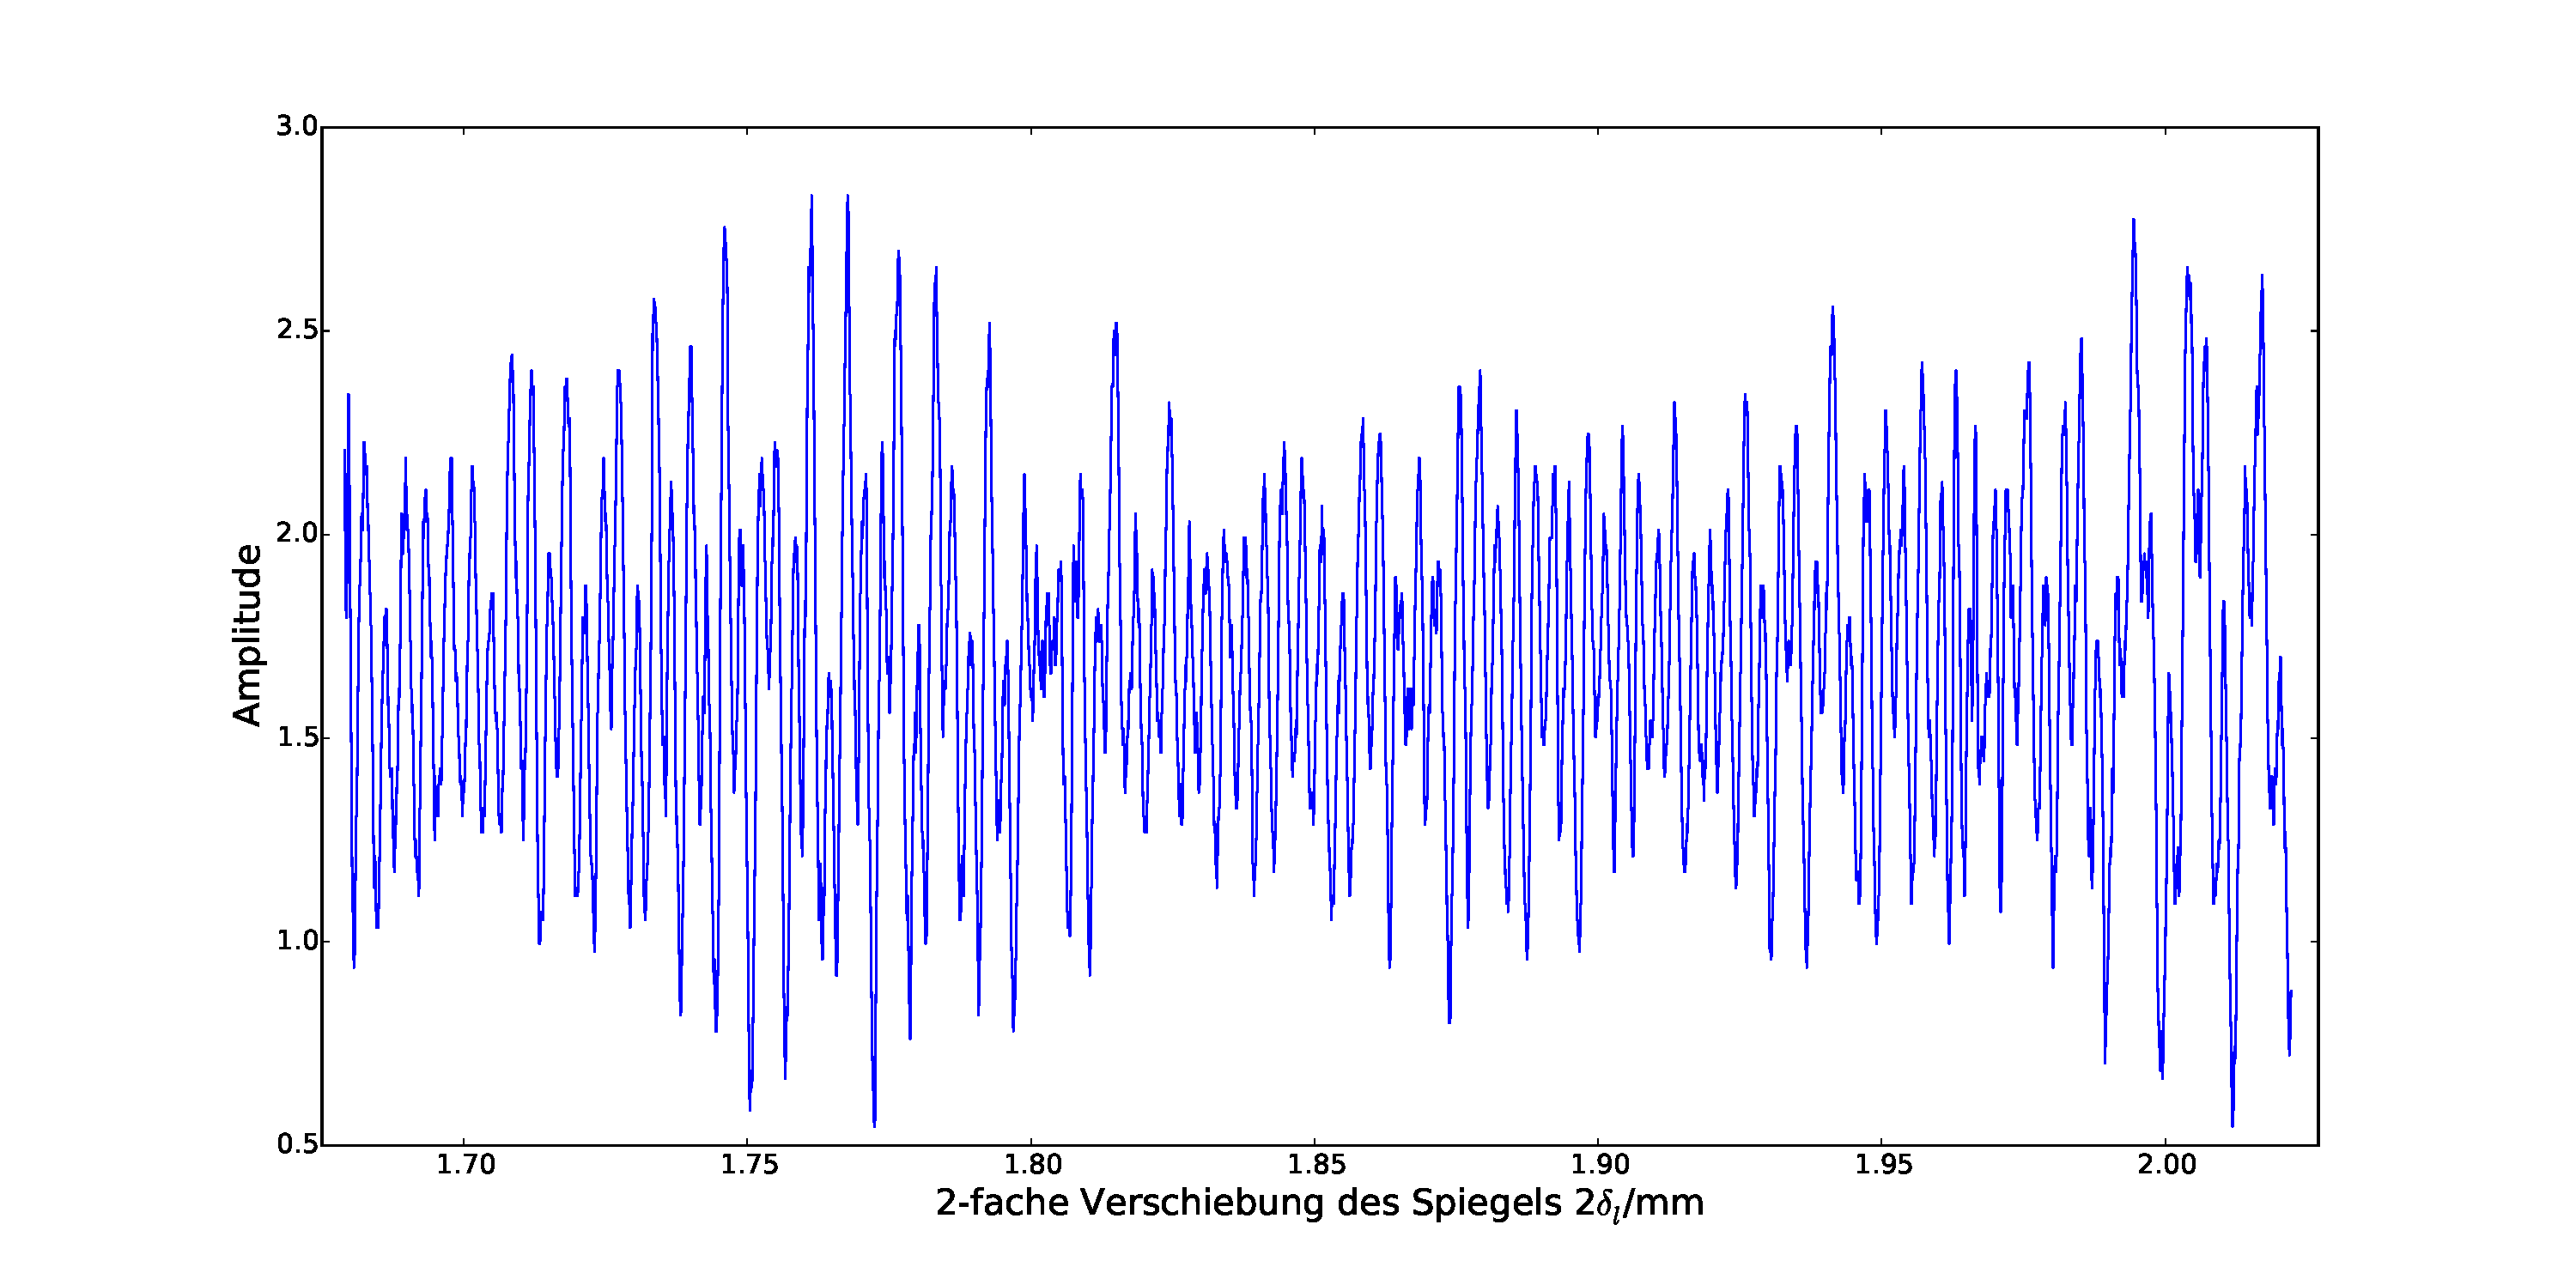
\includegraphics[scale = 0.38, clip = true, trim = 3cm 0cm 3cm 0cm]{Schwebung_Daten}
\caption{Schwebungsinterferogramm}
\label{fig:schwebungsinterferogramm}
\end{figure}
Da die Wellenl�nge der in dem Interferogramm erkennbaren Schwebung sehr stark von der erwarteten Schwebungswellenl�nge abweicht, wird es hier vorgezogen, einen FFT-Algorithmus (Fast-Fourier-Transform) f�r die diskrete Fouriertransformation zu verwenden, um herauszufinden, welche Wellenzahlen (1/$\lambda$) in dem Interferogramm vertreten sind. Auf eine Herleitung der DFT und deren Anwendung in der Analyse von Daten wird verzichtet, da dies lediglich einer Diskretisierung der Fouriertransformation entspricht, wodurch 'gesamplete' Messdaten und deren Frequenzen analysiert werden k�nnen. Die diskrete Fouriertransformation ist f�r die Analyse periodischer Signale geeignet, sodass bei der Analyse nichtperiodischer Signale hochfrequente Anteile in der Fouriertransformation hinzukommen, welche in den niedrigfrequenten Bereich gespiegelt werden, da $f(t)=e^{2\pi i nt/N}$ keine reelle Funktion ist. Dadurch sind die Daten nach der FFT stark verrauscht. Diese sind in Abbildung \ref{fig:fftschwebungsinterferogramm_ohne_fenster} dargestellt.
\begin{figure}[H]
\centering
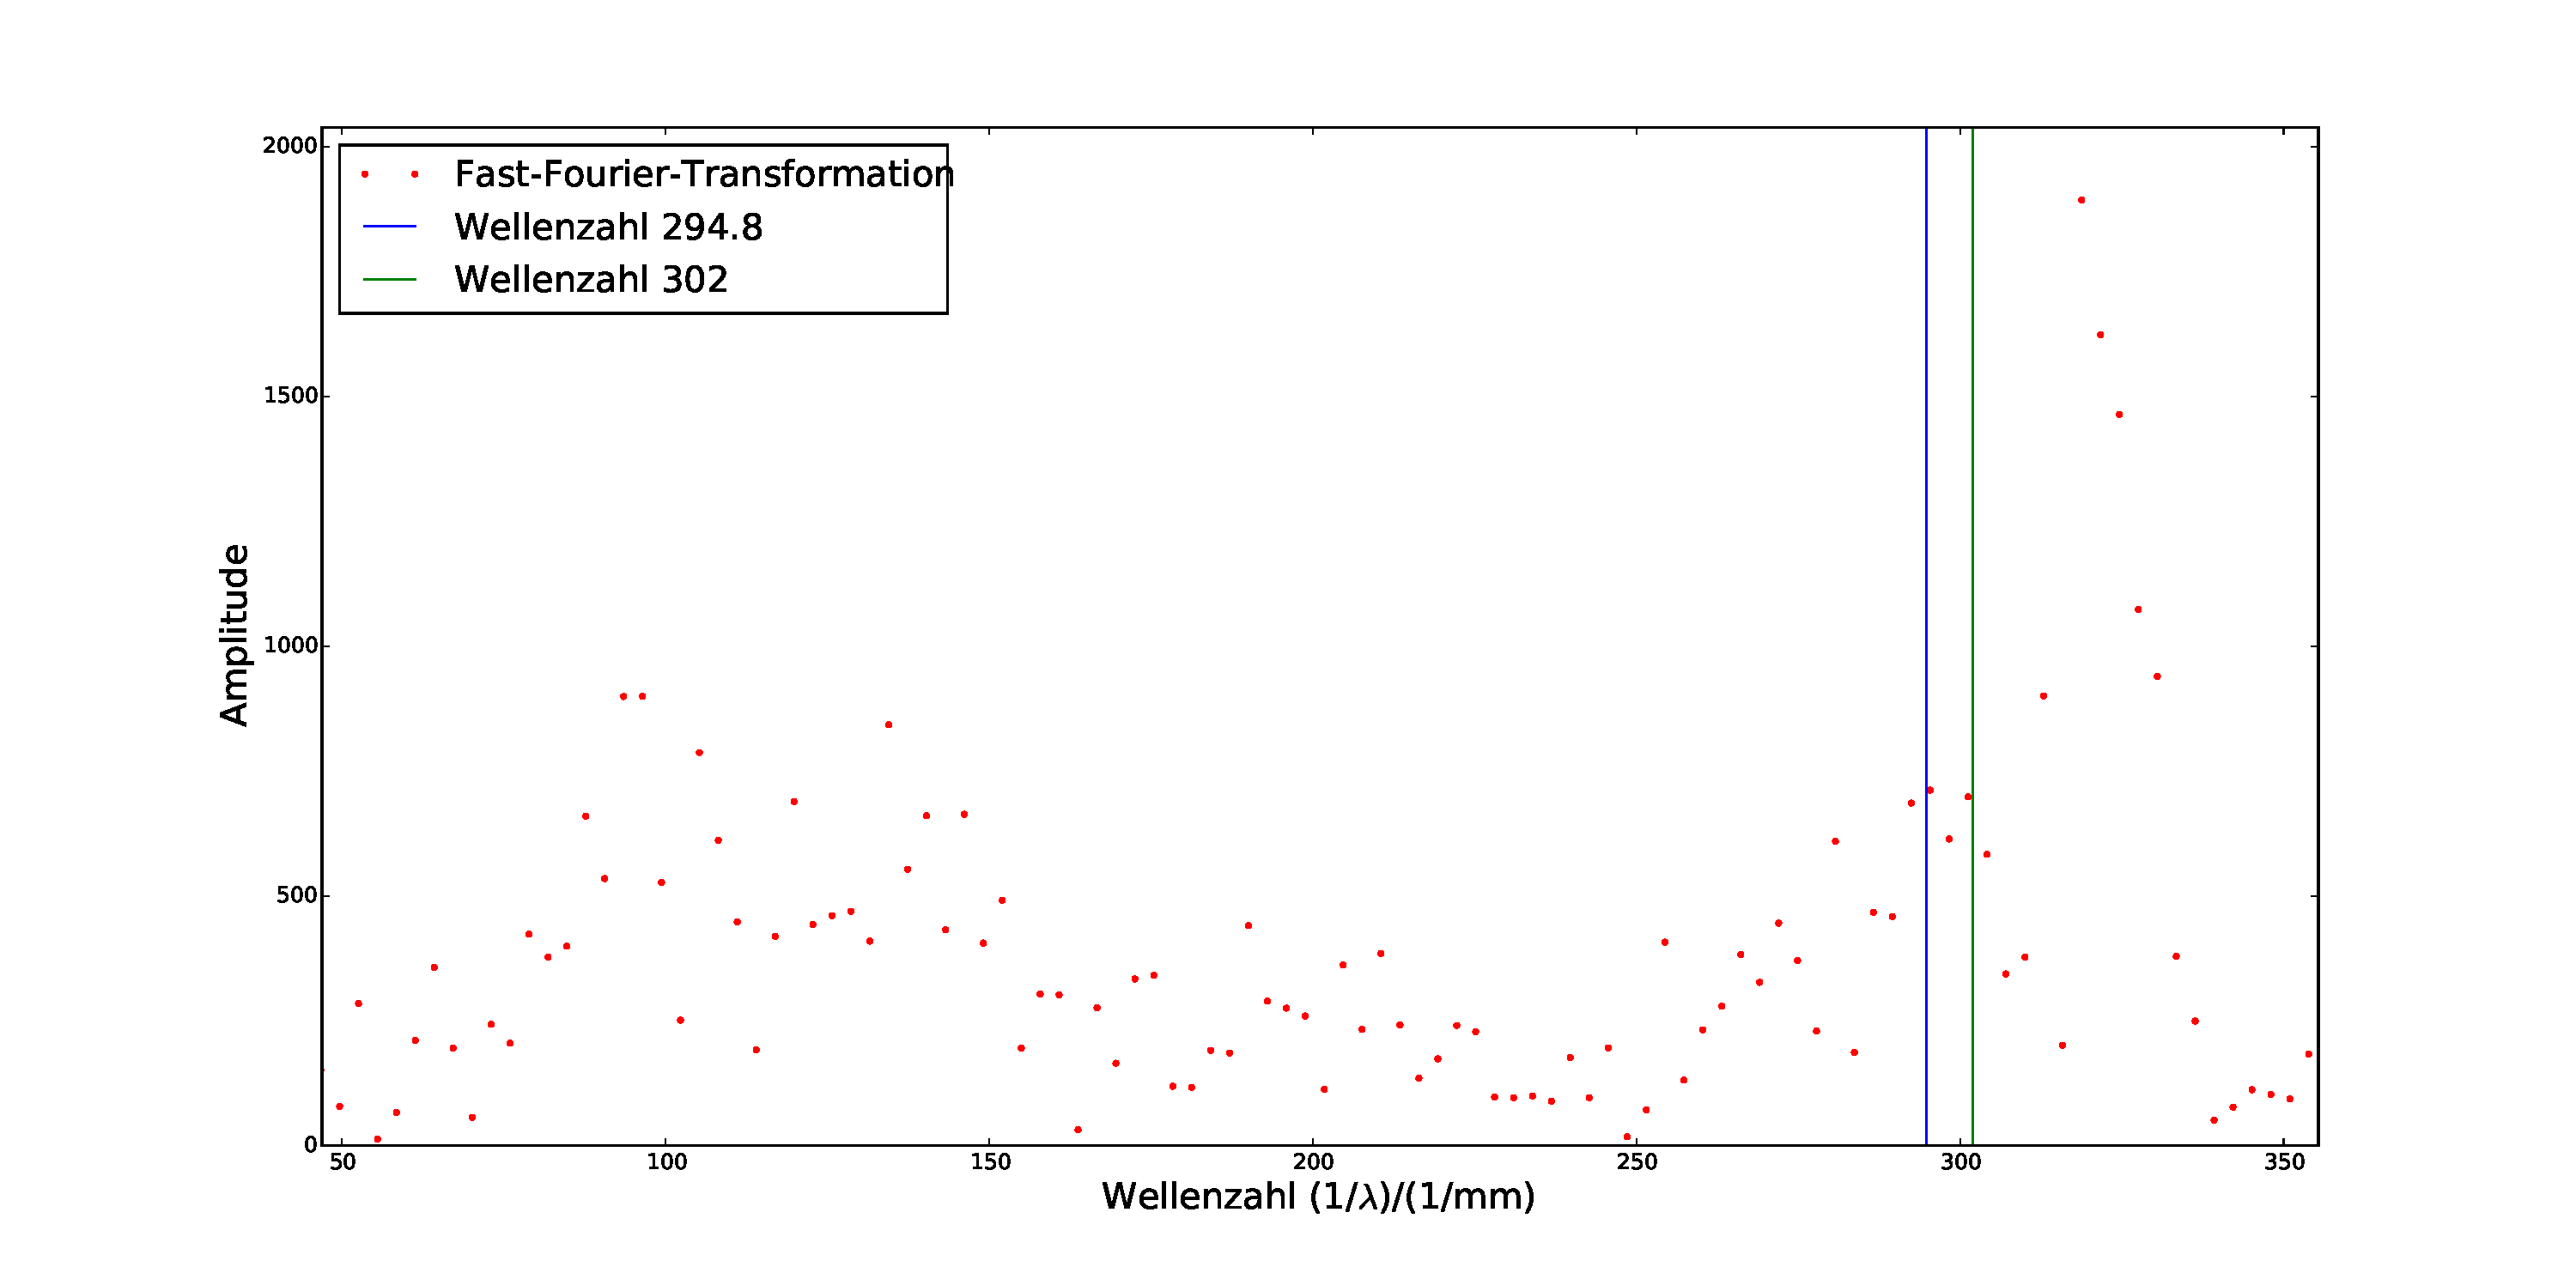
\includegraphics[scale = 0.38, clip = true, trim = 3cm 0cm 3cm 0cm]{Wellenzahlen50-350SchwebungohneFenster}
\caption{Diskrete Fouriertransformation des Schwebungsinterferogramms f�r Wellenzahlen ($1/\lambda$) von \SI{50}{$\frac{1}{mm}$} bis \SI{350}{$\frac{1}{mm}$}  ohne Fensterfunktion (verrauscht)}
\label{fig:fftschwebungsinterferogramm_ohne_fenster}
\end{figure}
Um die vertretenen Wellenzahlen aus dem Interferogramm abzulesen, wurde der Bereich \SI{260}{$\frac{1}{mm}$} bis \SI{340}{$\frac{1}{mm}$} n�her untersucht. Dieser ist in Abbildung \ref{fig:fftschwebungsinterferogramm} zu sehen.
\begin{figure}[H]
\centering
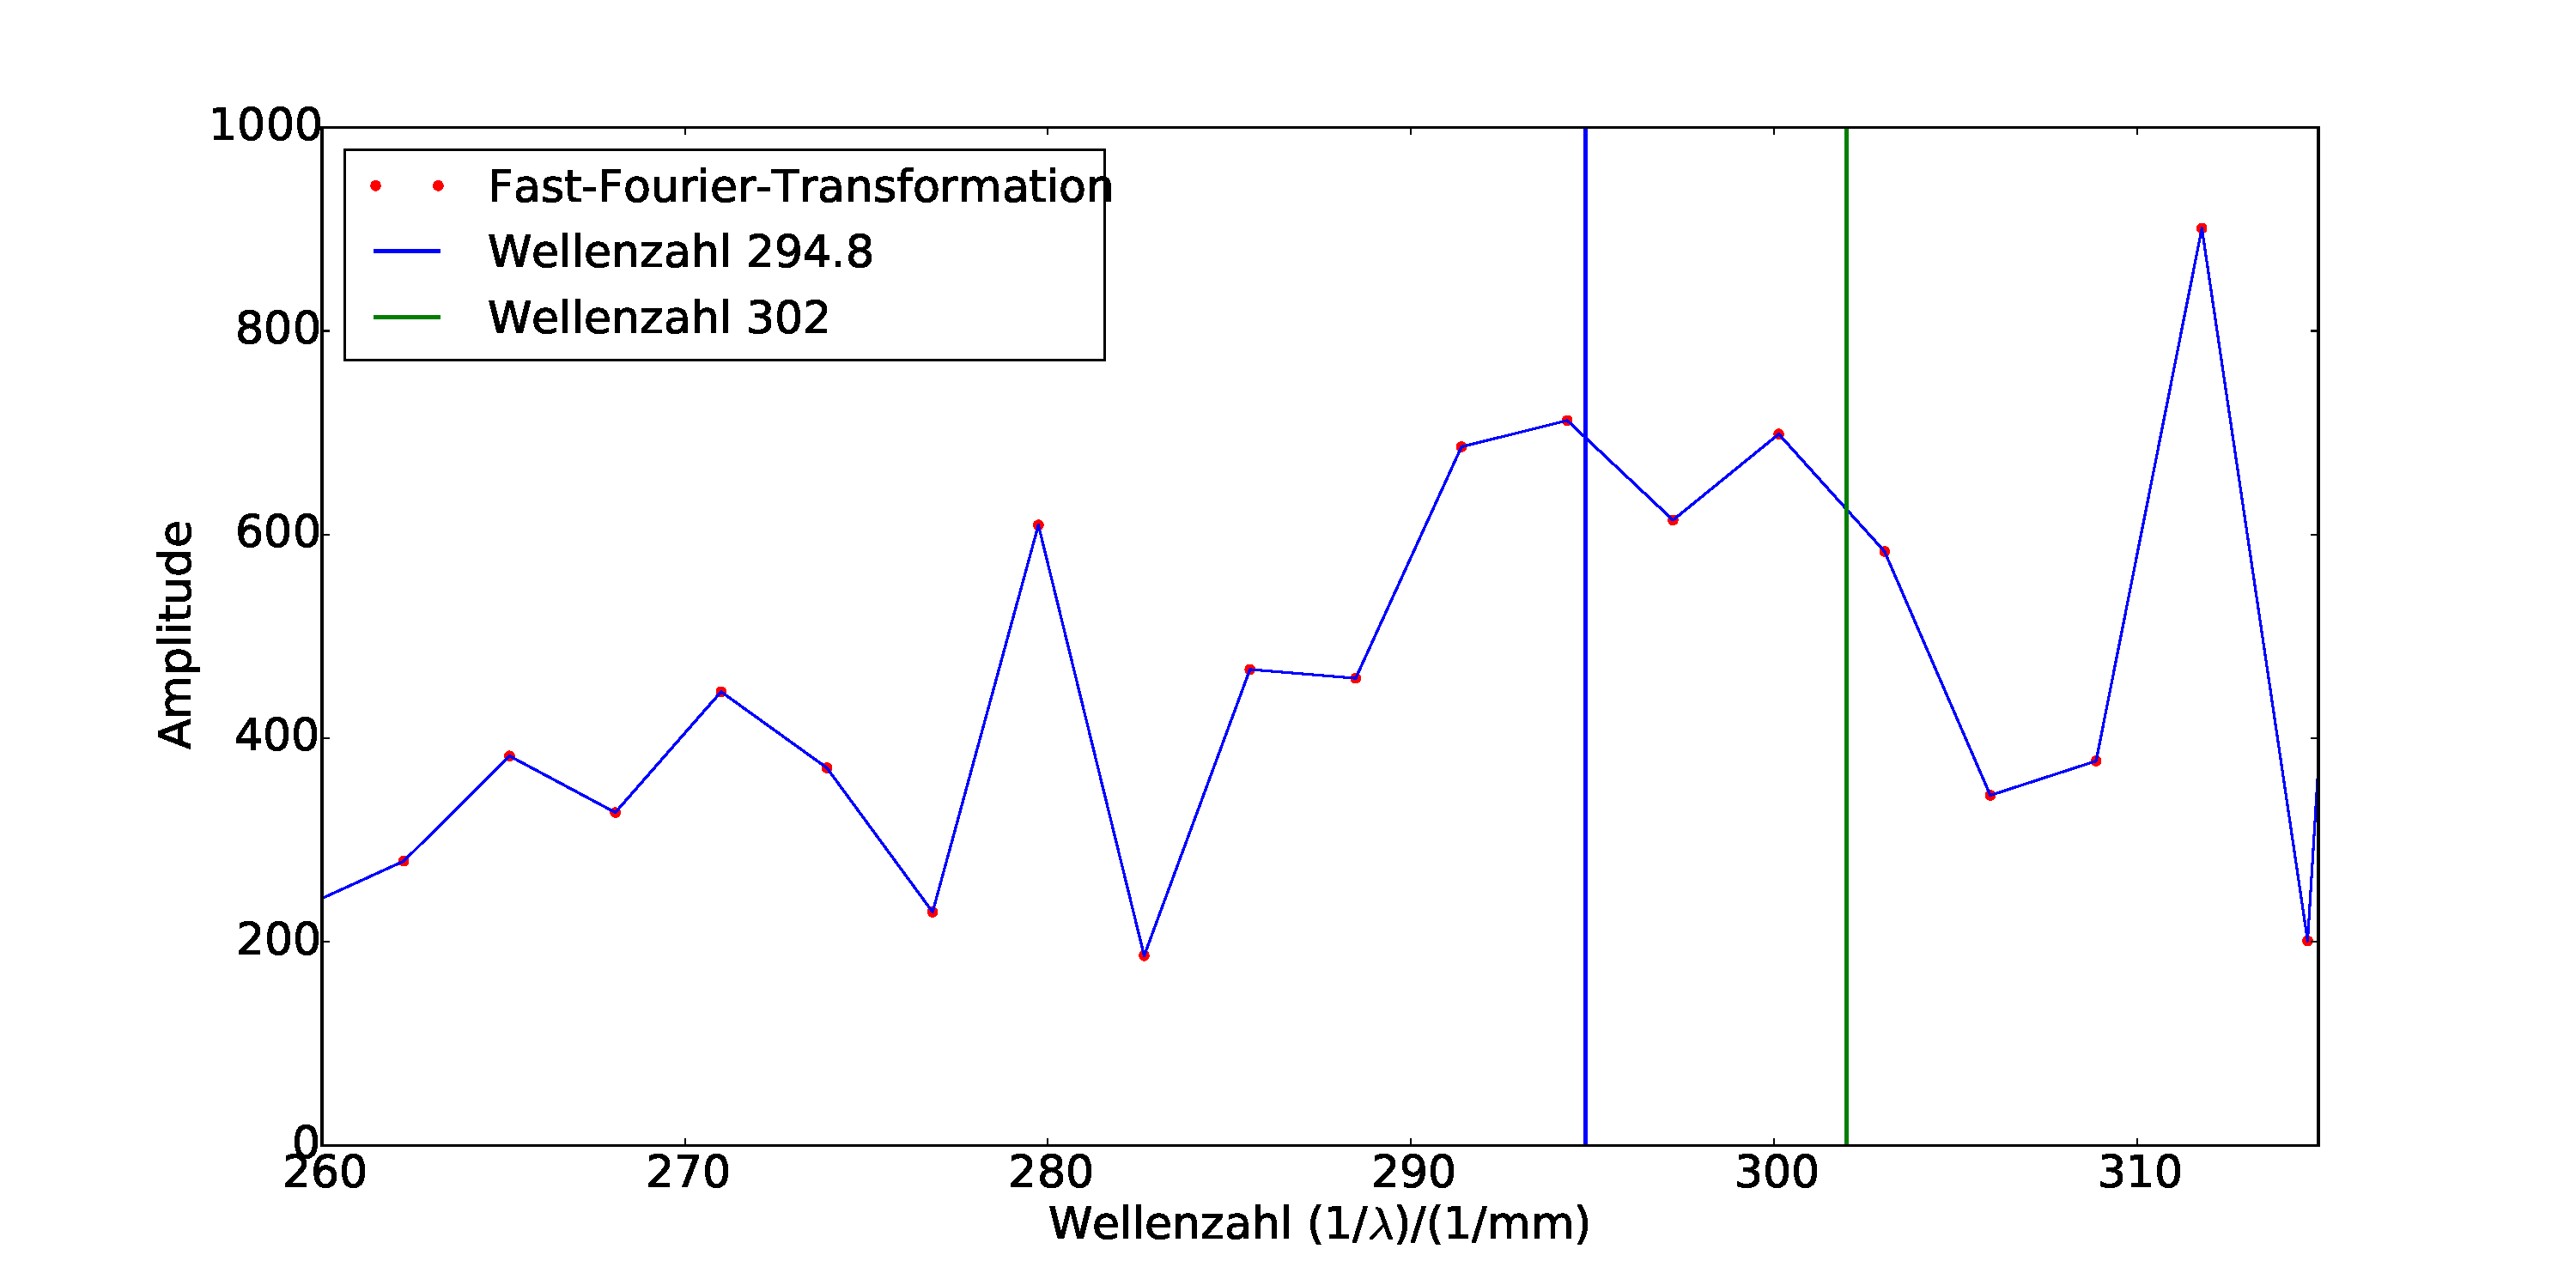
\includegraphics[scale = 0.38, clip = true, trim = 3cm 0cm 3cm 0cm]{Wellenzahlen260-340SchwebungohneFenster}
\caption{Diskrete Fouriertransformation des Schwebungsinterferogramms f�r Wellenzahlen ($1/\lambda$) von \SI{260}{$\frac{1}{mm}$} bis \SI{340}{$\frac{1}{mm}$}  ohne Fensterfunktion (verrauscht)}
\label{fig:fftschwebungsinterferogramm}
\end{figure}
Man sieht, dass die Wellenzahlen \SI{294,8(10)}{$\frac{1}{mm}$} und \SI{302(2)}{$\frac{1}{mm}$}, welche den Wellenl�ngen \SI{3,392(12)}{$\mu$m} und \SI{3,31(2)}{$\mu$m} entsprechen, in dem Interferogramm vertreten sind. Diese weichen von den erwarteten Wellenl�ngen \SI{3,31}{$\mu$m} und \SI{3,39}{$\mu$m} um \SI{0}{\percent} bzw. \SI{0,05}{\percent} ab. Daneben sind andere Frequenzen st�rker in dem Interferogramm vertreten.
Um herauszufinden, ob diese durch die Nichtperiodizit�t zustandekommen, multipliziert man sogenannte Fensterfunktionen mit dem Interferogramm, welche das Signal 'sanft' ein und ausblenden. In diesem Fall wurde die Funktion $f(x)=(\frac{1-\cos(\frac{2 \pi x}{L})}{2})^k$, wobei L die L�nge des Interferogramms ist und $k$ eine nat�rliche Zahl, als Fensterfunktion gew�hlt. Dadurch wird das Signal periodisch und das Rauschen durch Randeffekte kleiner. Abh�ngig von der Gr��e $k$, wirde der mittlere Teil des Interferogramms unterschiedlich stark gewichtet. Deshalb wurden f�r $k$ die Werte 1, 4 und 10 eingesetzt. Die Spektren f�r den Wellenzahlbereich von \SI{50}{$\frac{1}{mm}$} bis \SI{350}{$\frac{1}{mm}$} sind in Abbildung \ref{fig:fftschwebungsinterferogramm_k_1} ($k=1$), \ref{fig:fftschwebungsinterferogramm_k_4} ($k=4$) und \ref{fig:fftschwebungsinterferogramm_k_10} ($k=10$) dargestellt.
\begin{figure}[H]
\centering
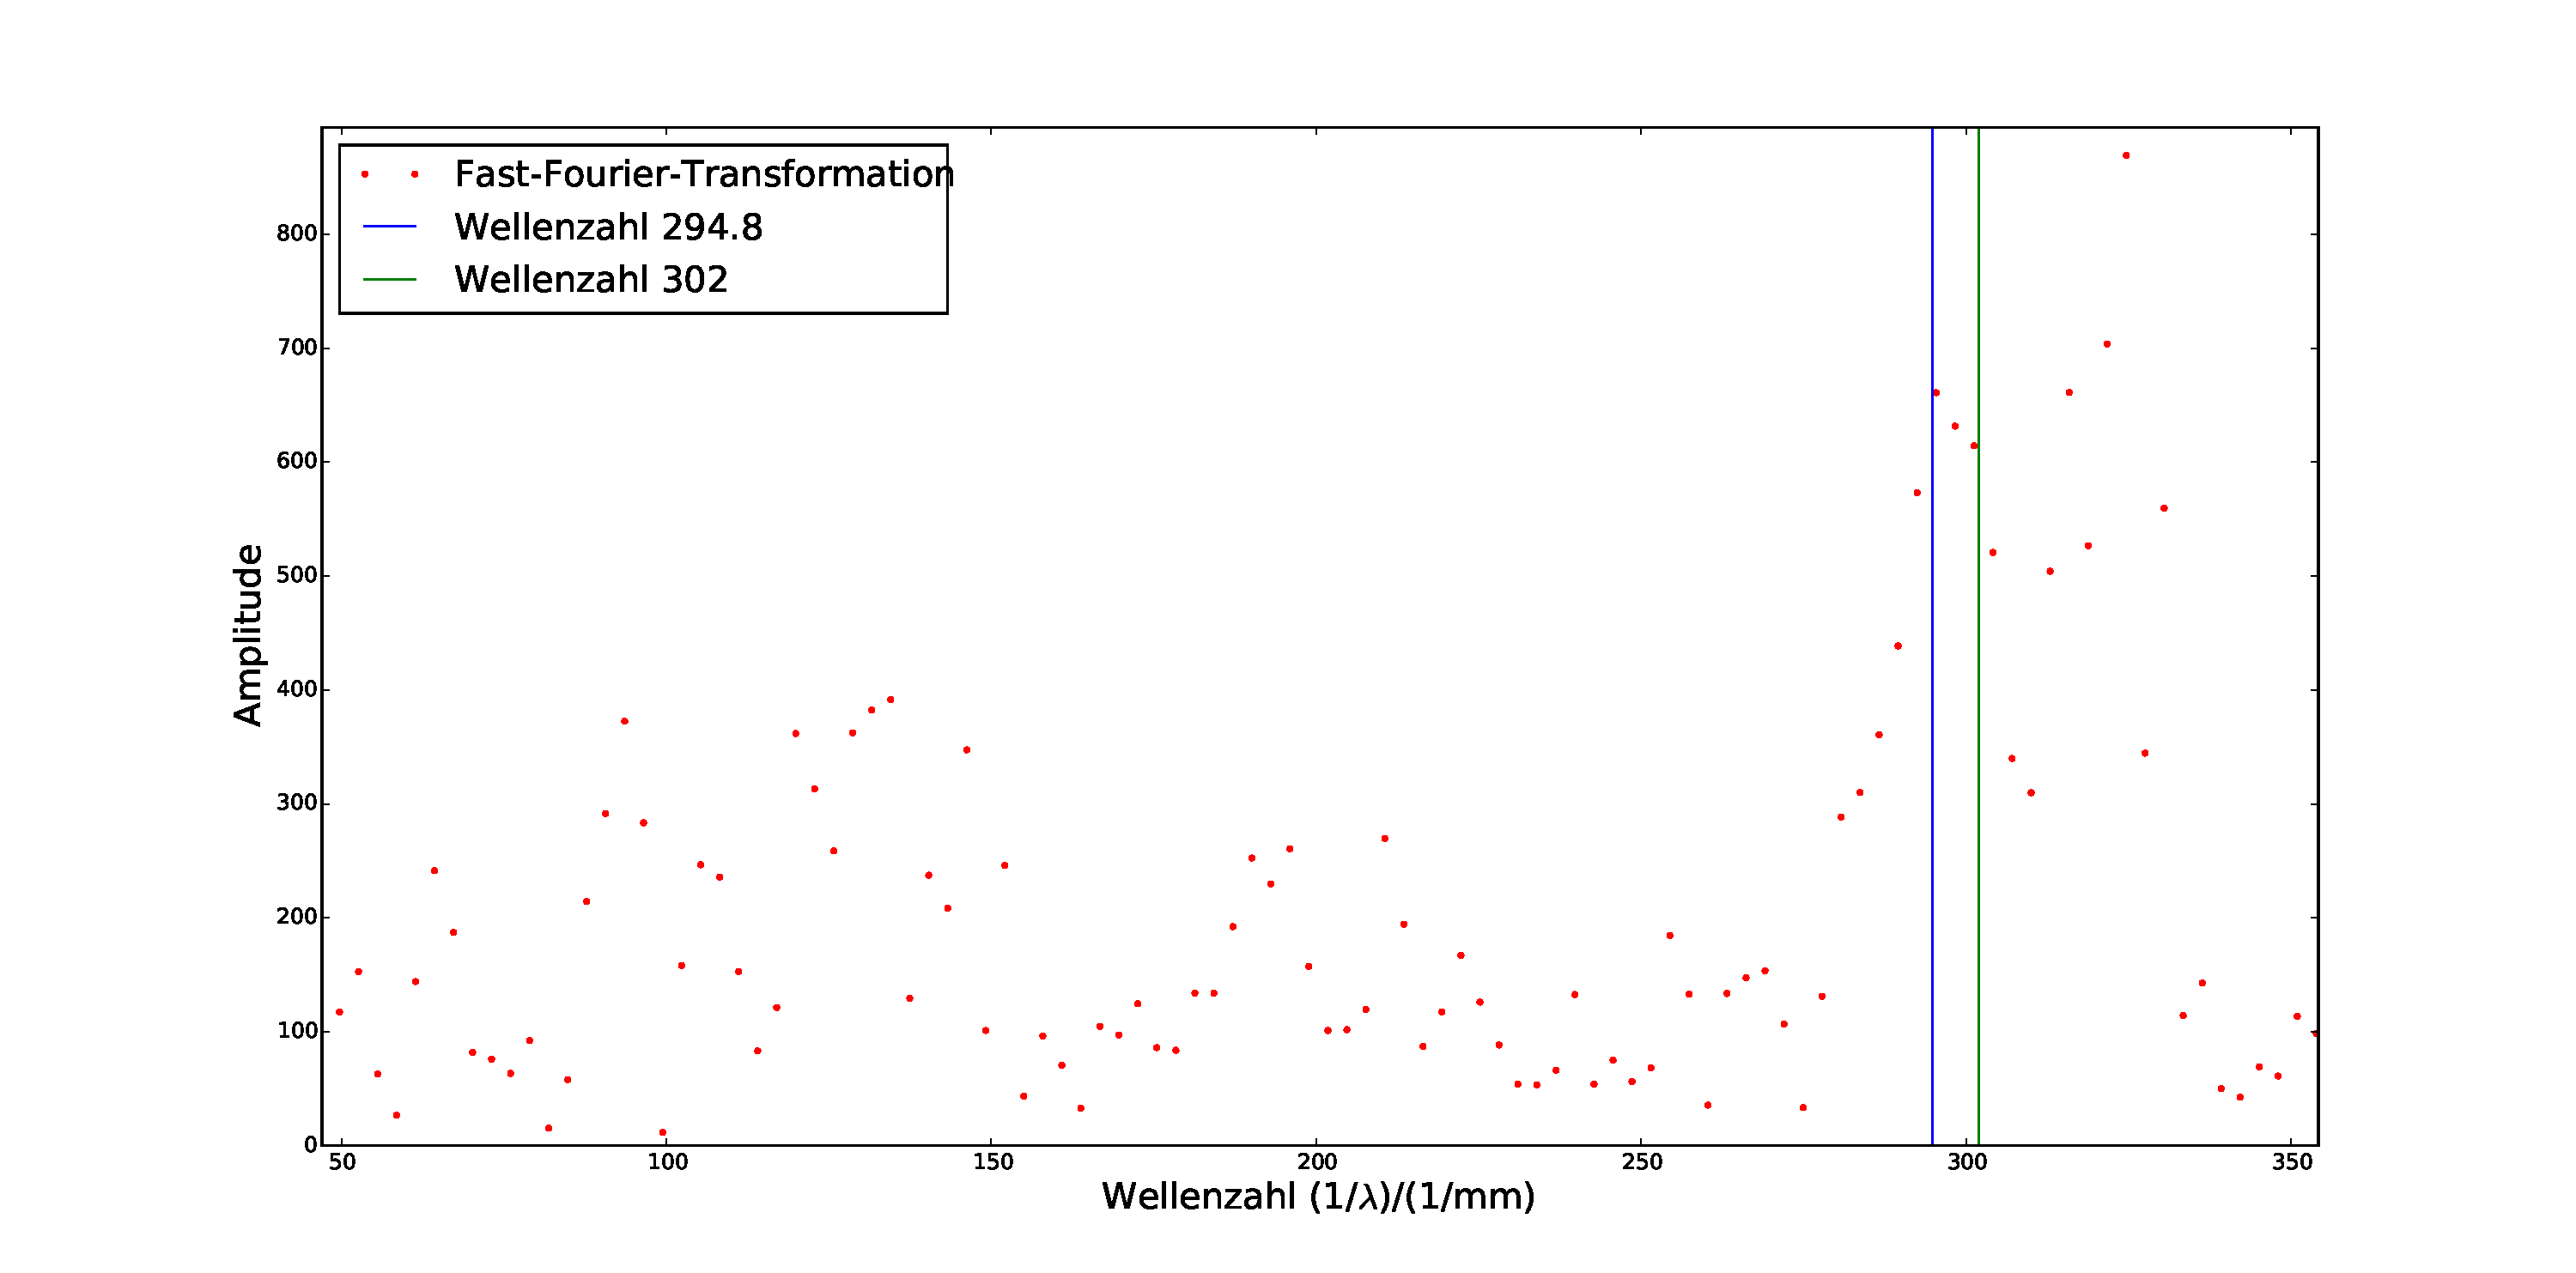
\includegraphics[scale = 0.38, clip = true, trim = 3cm 0cm 3cm 0cm]{Wellenzahlen50-350SchwebungmitFenster(0,5*(1-cos))}
\caption{Diskrete Fouriertransformation des Schwebungsinterferogramms f�r Wellenzahlen ($1/\lambda$) von \SI{50}{$\frac{1}{mm}$} bis \SI{360}{$\frac{1}{mm}$} mit Fensterfunktion $f(x)=(\frac{1-\cos(\frac{2 \pi x}{L})}{2})$}
\label{fig:fftschwebungsinterferogramm_k_1}
\end{figure}
\begin{figure}[H]
\begin{subfigure}[t]{0.49\textwidth}
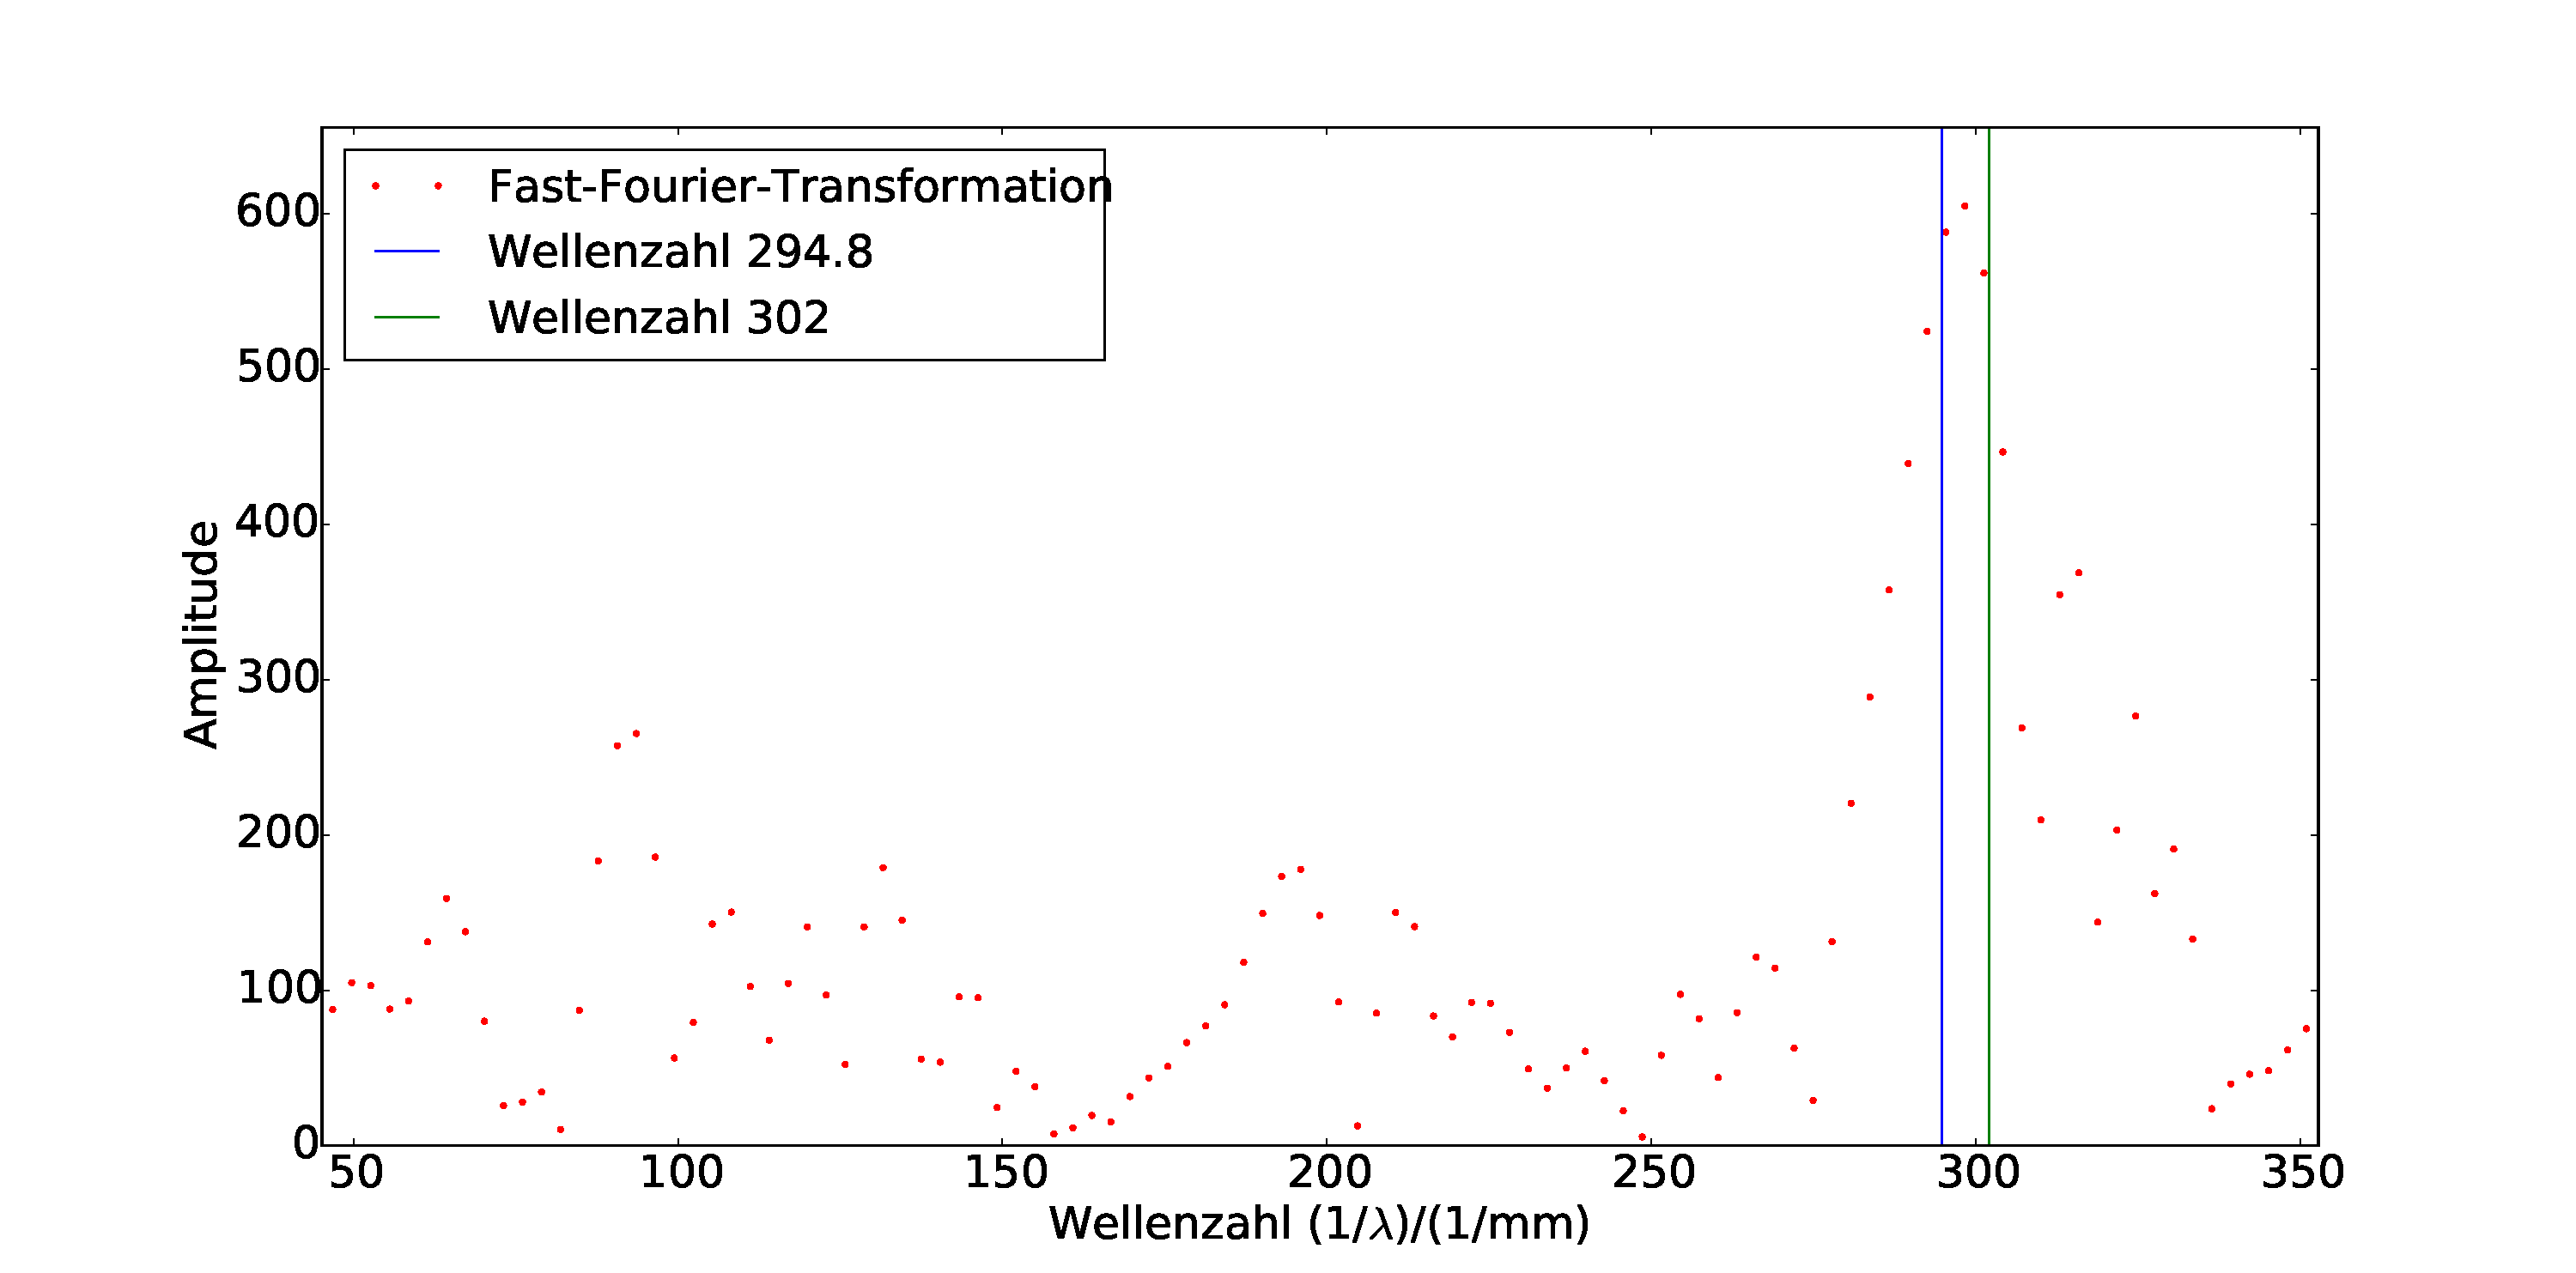
\includegraphics[scale = 0.19, clip = true, trim = 3cm 0cm 3cm 0cm]{Wellenzahlen50-350SchwebungmitFenster(0,5*(1-cos))**4}
\caption{Diskrete Fouriertransformation des Schwebungsinterferogramms f�r Wellenzahlen ($1/\lambda$) von \SI{50}{$\frac{1}{mm}$} bis \SI{360}{$\frac{1}{mm}$} mit Fensterfunktion\\$f(x)=(\frac{1-\cos(\frac{2 \pi x}{L})}{2})^4$}
\label{fig:fftschwebungsinterferogramm_k_4}
\end{subfigure}
\hspace{0.02\textwidth}
\begin{subfigure}[t]{0.49\textwidth}
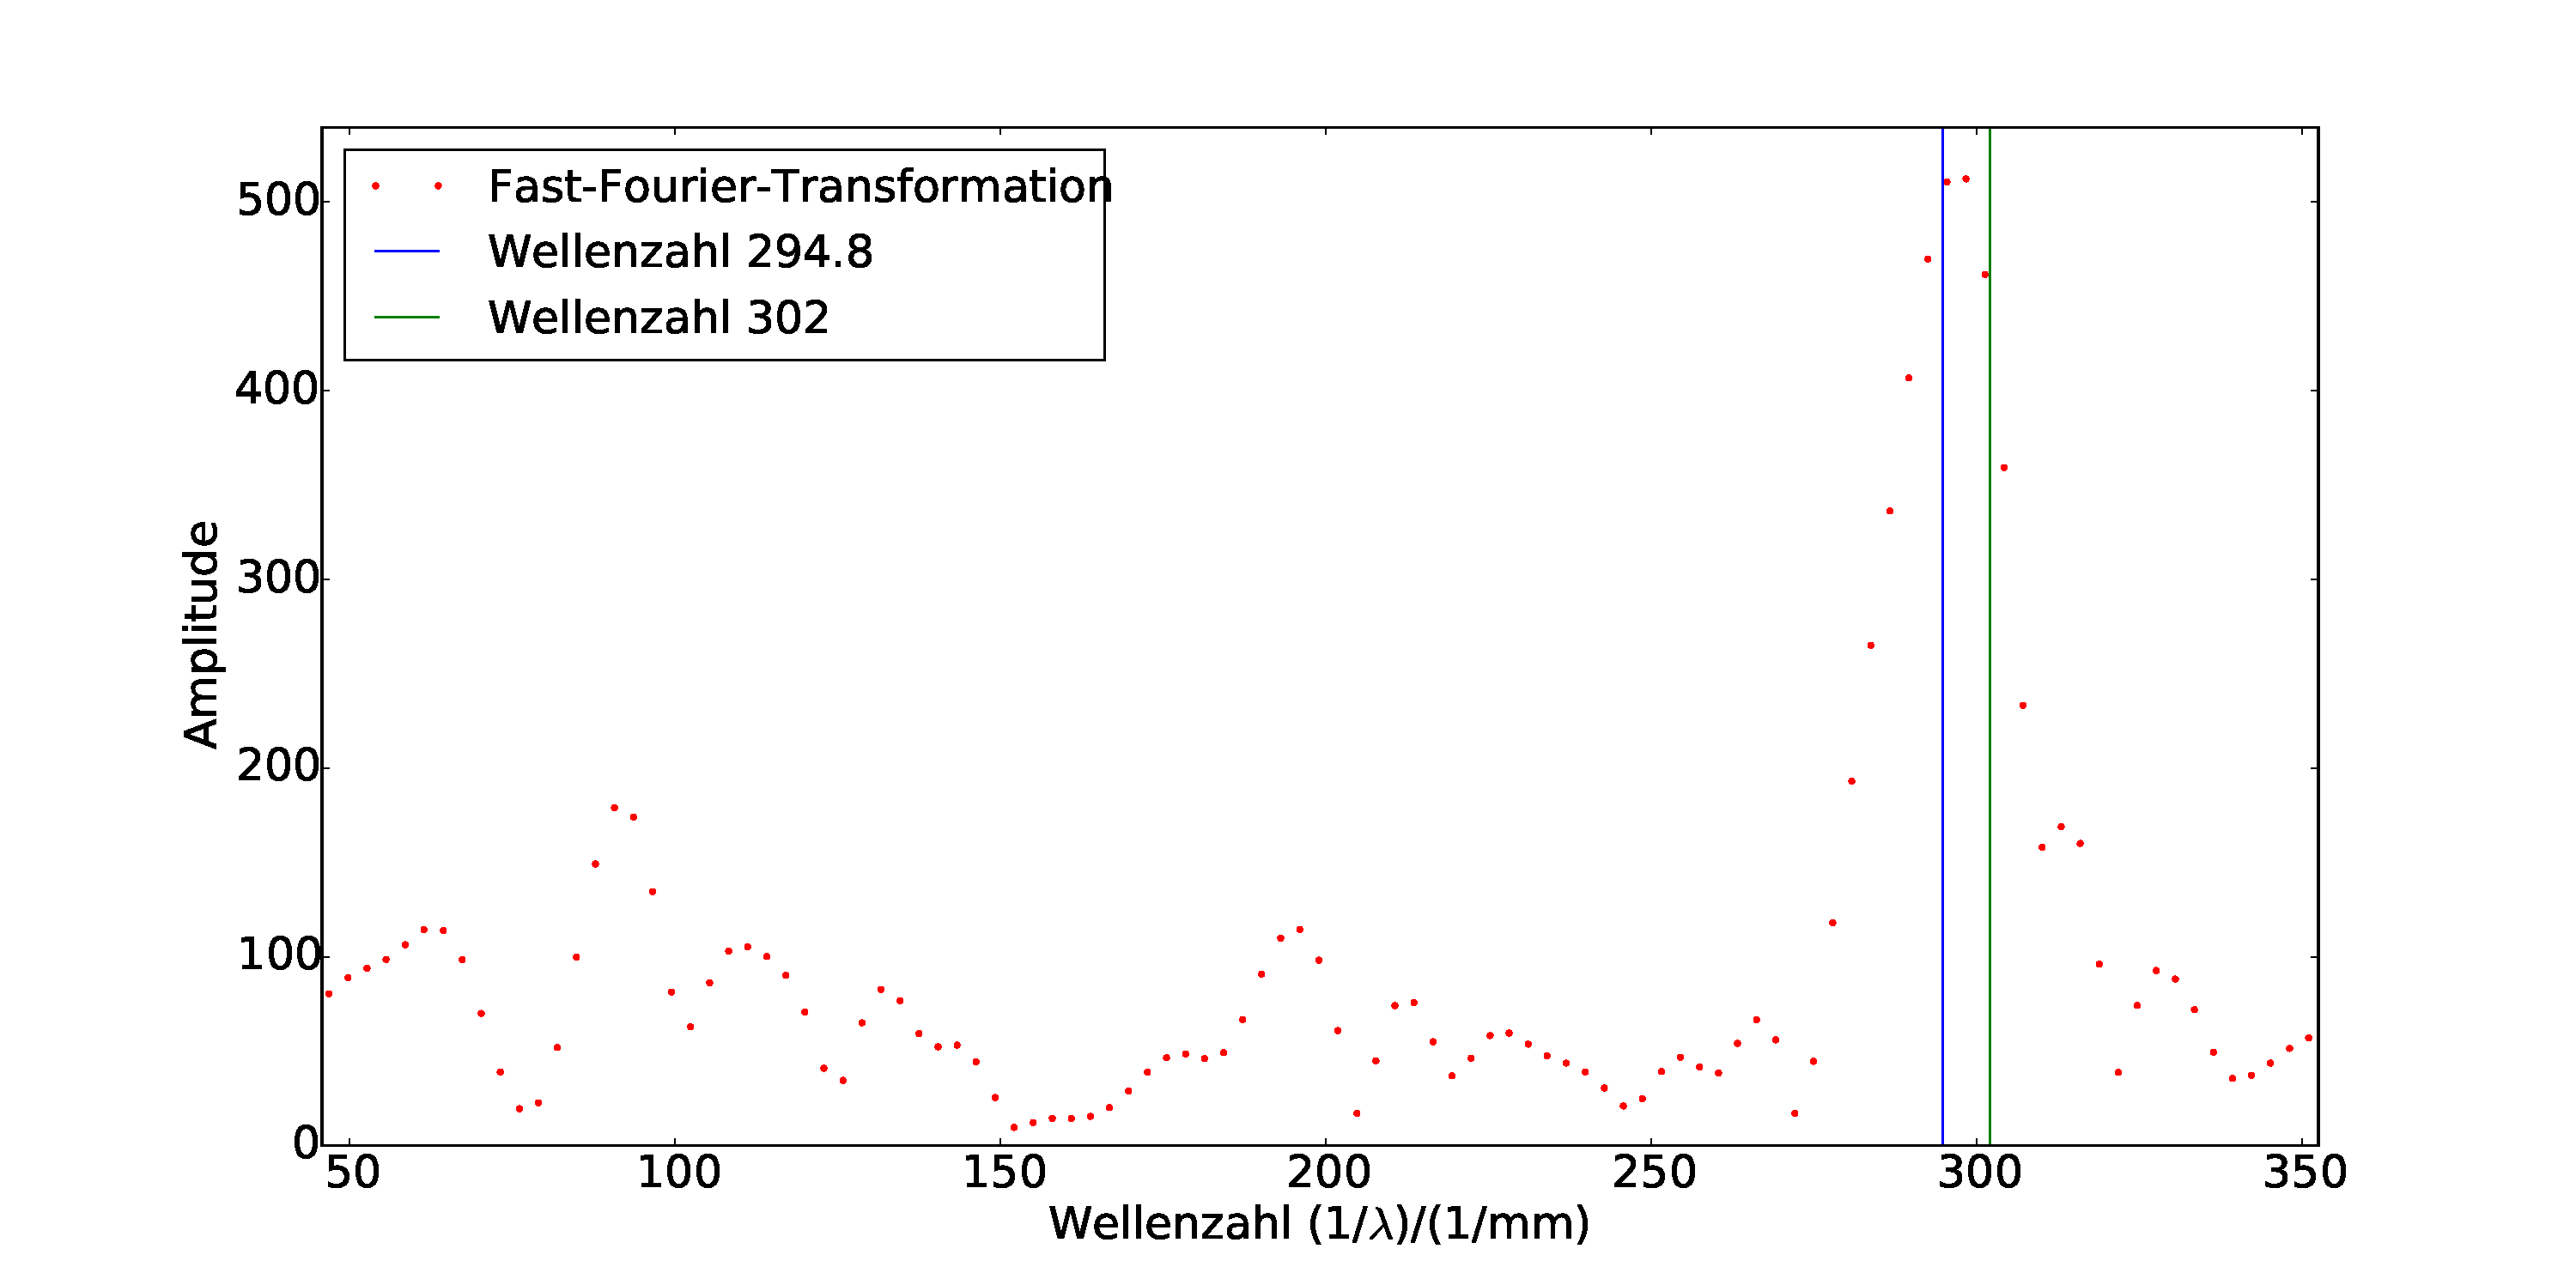
\includegraphics[scale = 0.19, clip = true, trim = 3cm 0cm 3cm 0cm]{Wellenzahlen50-350SchwebungmitFenster(0,5*(1-cos))**10}
\caption{Diskrete Fouriertransformation des Schwebungsinterferogramms f�r Wellenzahlen ($1/\lambda$) von \SI{50}{$\frac{1}{mm}$} bis \SI{360}{$\frac{1}{mm}$} mit Fensterfunktion\\$f(x)=(\frac{1-\cos(\frac{2 \pi x}{L})}{2})^{10}$}
\label{fig:fftschwebungsinterferogramm_k_10}
\end{subfigure}
\end{figure}
Man sieht, dass das Rauschen mit h�herem $k$ geringer wird, sodass die erwarteten Wellenzahlen bereits bei $k = 4$ die gr��te Amplitude im gesamten Interferogramm besitzen. Die beiden Peaks bei \SI{294,8(10)}{$\frac{1}{mm}$} und \SI{302(2)}{$\frac{1}{mm}$} verschmieren mit gr��er werdendem k zu einem Peak, sodass bei $k=10$ die Peaks nichtmehr voneinander unterschieden werden k�nnen. Trotzdem sieht man, dass das Rauschen bei $k=10$ am besten unterdr�ckt wird, sodass andere Wellenzahlen eine sehr geringe Amplitude besitzen. Daneben kann man Infrarotwellenzahlen von Plankstrahlern bei Raumtemperatur bei ca. \SI{100}{$\frac{1}{mm}$} in den letzten beiden Plots gut erkennen, welche ebenfalls nicht als Rauschen herausgefiltert werden. Diese Tatsache unterst�tzt die Konsistenz dieses Resultates. Zusammenfassend konnten die gefundenen Wellenl�ngen bei \SI{3,392(12)}{$\mu$m} und \SI{3,31(2)}{$\mu$m} per FFT mit relativ gro�er Genauigkeit durch die Benutzung von Fensterfunktionen bestimmt werden, wobei der Peak bei der Wellenl�nge \SI{3,31(2)}{$\mu$m} abh�ngig von der Fensterfunktion nicht mehr zu erkennen ist.